\documentclass[a4paper]{article}
\usepackage{enumitem}
\usepackage[english]{babel}
\usepackage[utf8]{inputenc}
\usepackage{amsmath}
\newcommand{\verbatimfont}[1]{\renewcommand{\verbatim@font}{\ttfamily#1}}
\usepackage{graphicx}
\usepackage[colorinlistoftodos]{todonotes}
\usepackage[margin=0.25in]{geometry}
\usepackage{lscape}
\title{Advanced Networking Lab 5: OpenFlow}

\author{Fouad Makioui \& Kotaiba Alachkar}



\date{\today}

\begin{document}
\maketitle


\section{Task 1: Deployment of the OpenFlow controller}
\label{sec:task1}

Downloading the file
\begin{verbatim}
    wget https://github.com/floodlight/floodlightrchive/v1.2.tar.gz
\end{verbatim}
installing ant and openjdk
\begin{verbatim}
    sudo apt-get install ant
    sudo apt-get install openjdk-9-jdk-headless
\end{verbatim}
unpacking tar file
\begin{verbatim}
    tar -xvf v1.2.tar.gz
\end{verbatim}
compiling floodlight
starting floodlight
\begin{verbatim}
    java -jar target/floodlight.jar
\end{verbatim}

Accept connections to port 6653 only from OS3 network.
\begin{verbatim}
    sudo ufw allow from 145.100.0.0/16  to any port 6653
\end{verbatim}





\section{Task 2: Network Setup}
\label{sec:task2}

We connected Fouad's server (Reims) to AN2018 Openflow switch at port 11.
eno2 IP: 
USB-interface IP: 10.0.1.83/24
commands used to configure the usb ethernet device
\begin{verbatim}
root@reims:/home/fmakioui# ip address add 10.0.1.83/24 dev enxd46e0e0891e9
root@reims:/home/fmakioui# ifconfig enxd46e0e0891e9 up
\end{verbatim}


Configuration:

\begin{verbatim}
    
ovs-vsctl add-br br_11 -- set bridge br_11 datapath_type=pica8
ovs-vsctl add-port br_11 ge-1/1/11 vlan_mode=trunk tag=1 -- set interface ge-1/1/11 type=pica8
ovs-vsctl add-port br_11 ge-1/1/8 vlan_mode=trunk tag=1 -- set interface ge-1/1/8 type=pica8
    
ovs-vsctl show
e4846a95-7489-41ac-a935-e75eba7cf6b1
    Bridge "br_4"
        Port "ge-1/1/14"
            Interface "ge-1/1/14"
        Port "ge-1/1/13"
            Interface "ge-1/1/13"
        Port "br_4"
            Interface "br_4"
                type: internal
    Bridge "br_1"
        Controller "tcp:10.0.1.191:6653"
        Port "te-1/1/21"
            Interface "te-1/1/21"
        Port "te-1/1/22"
            Interface "te-1/1/22"
        Port "ge-1/1/22"
            Interface "ge-1/1/22"
        Port "br_1"
            Interface "br_1"
                type: internal
        Port "ge-1/1/21"
            Interface "ge-1/1/21"
    Bridge "br_6"
        Port "ge-1/1/42"
            Interface "ge-1/1/42"
        Port "br_6"
            Interface "br_6"
                type: internal
        Port "ge-1/1/41"
            Interface "ge-1/1/41"
    Bridge "br_2"
        Port "br_2"
            Interface "br_2"
                type: internal
    Bridge "br_9"
        Port "br_9"
            Interface "br_9"
                type: internal
    Bridge "br_11"
        Port "ge-1/1/8"
            tag: 1
            Interface "ge-1/1/8"
                type: "pica8"
        Port "ge-1/1/11"
            tag: 1
            Interface "ge-1/1/11"
                type: "pica8"
        Port "br_11"
            Interface "br_11"
                type: internal
\end{verbatim}
 

Monitor the port status and examine the port configuration with ovs-ofctl show br\_11 command:

\begin{verbatim}
ovs-ofctl show br_11
OFPT_FEATURES_REPLY (OF1.4) (xid=0x2): dpid:e3ba089e01e99512
n_tables:254, n_buffers:256
capabilities: FLOW_STATS TABLE_STATS PORT_STATS GROUP_STATS
OFPST_PORT_DESC reply (OF1.4) (xid=0x4):
 8(ge-1/1/8): addr:08:9e:01:e9:95:12
     config:     0
     state:      LINK_UP
     current:    1GB-FD COPPER AUTO_NEG
     advertised: 10MB-HD 10MB-FD 100MB-HD 100MB-FD 1GB-FD COPPER AUTO_NEG
     supported:  10MB-HD 10MB-FD 100MB-HD 100MB-FD 1GB-FD COPPER AUTO_NEG
     peer:       10MB-HD 10MB-FD 100MB-HD 100MB-FD 1GB-FD COPPER
     speed: 1000 Mbps now, 1000 Mbps max
 11(ge-1/1/11): addr:08:9e:01:e9:95:12
     config:     0
     state:      LINK_UP
     current:    1GB-FD COPPER AUTO_NEG
     advertised: 10MB-HD 10MB-FD 100MB-HD 100MB-FD 1GB-FD COPPER AUTO_NEG
     supported:  10MB-HD 10MB-FD 100MB-HD 100MB-FD 1GB-FD COPPER AUTO_NEG
     peer:       10MB-HD 10MB-FD 100MB-HD 100MB-FD 1GB-HD 1GB-FD COPPER
     speed: 1000 Mbps now, 1000 Mbps max
 LOCAL(br_11): addr:08:9e:01:e9:95:12
     config:     0
     state:      LINK_UP
     current:    10MB-FD COPPER
     supported:  10MB-FD COPPER
     speed: 10 Mbps now, 10 Mbps max
OFPT_GET_CONFIG_REPLY (OF1.4) (xid=0x6): frags=normal miss_send_len=
\end{verbatim}


Configure the bridge to connect to the controller:

\begin{verbatim}
    ovs-vsctl set-controller br_11 tcp:10.0.1.83:6653
     
     Check
     Bridge "br_11"
        Controller "tcp:10.0.1.83:6653"
        Port "ge-1/1/8"
            tag: 1
            Interface "ge-1/1/8"
                type: "pica8"
        Port "ge-1/1/11"
            tag: 1
            Interface "ge-1/1/11"
                type: "pica8"
        Port "br_11"
            Interface "br_11"
                type: internal

ovs-vsctl -- set bridge br_11 protocols=OpenFlow11,OpenFlow12,OpenFlow13
\end{verbatim}



\section{Task 3: Basics}
\label{sec:task3}

\subsection{What happens to the flow table a few seconds after you stop the test? Why?}
We have configured our eno2 ethernet card with the following IP addresses.
Kotaiba IP address 10.1.1.8/24
Fouad IP address 10.1.1.1/24

We going to perform a ping from Kotaiba server to Fouad server 
(through our private IP addressing) from 10.1.1.8 to 10.1.1.1:


\begin{verbatim}
root@bristol:~# ping 10.1.1.1
PING 10.1.1.1 (10.1.1.1) 56(84) bytes of data.
64 bytes from 10.1.1.1: icmp_seq=4 ttl=64 time=145 ms
64 bytes from 10.1.1.1: icmp_seq=5 ttl=64 time=26.4 ms
64 bytes from 10.1.1.1: icmp_seq=6 ttl=64 time=0.177 ms
64 bytes from 10.1.1.1: icmp_seq=7 ttl=64 time=0.174 ms
64 bytes from 10.1.1.1: icmp_seq=8 ttl=64 time=0.177 ms
64 bytes from 10.1.1.1: icmp_seq=9 ttl=64 time=0.174 ms
64 bytes from 10.1.1.1: icmp_seq=10 ttl=64 time=0.176 ms
\end{verbatim}

During the ping we dumped the flow. below you can see the flow during the ping.

\begin{verbatim}
ovs-ofctl dump-flows br_11 
OFPST_FLOW reply (OF1.3) (xid=0x2):
 cookie=0x0, duration=187.214s, table=0, n_packets=n/a, n_bytes=0, priority=0 actions=CONTROLLER:65535
 cookie=0x20000000000000, duration=18.073s, table=0, n_packets=n/a, n_bytes=1326, idle_timeout=5, priority=1,ip,in_port=8,dl_src=d4:ae:52:bf:e4:db,dl_dst=34:17:eb:f0:e0:e0,nw_src=10.1.1.8,nw_dst=10.1.1.1 actions=output:11
 cookie=0x20000000000000, duration=18.043s, table=0, n_packets=n/a, n_bytes=1326, idle_timeout=5, priority=1,ip,in_port=11,dl_src=34:17:eb:f0:e0:e0,dl_dst=d4:ae:52:bf:e4:db,nw_src=10.1.1.1,nw_dst=10.1.1.8 actions=output:8
\end{verbatim}

After few seconds we stopped the ping, the following output are showed:

\begin{verbatim}
ovs-ofctl dump-flows br_11 
OFPST_FLOW reply (OF1.3) (xid=0x2):
 cookie=0x0, duration=189.293s, table=0, n_packets=n/a, n_bytes=0, priority=0 actions=CONTROLLER:65535
\end{verbatim}

The flow table contains information about the source and destination of the flow. 

\newpage
\section{Task 4: Packet Capture}
\subsection{1- The switch connects to the controller.}
We captured the traffic on Fouad's server with tshark and let tshark output the capture into a pcap format. After that we analyzed the traffic with Wireshark.

\begin{verbatim}
root@reims:/home/fmakioui# tshark -i enxd46e0e0891e9 -w ~/controller.pcap -F pcap
\end{verbatim}
\label{sec:task4}
\begin{figure}[h]
    \centering
    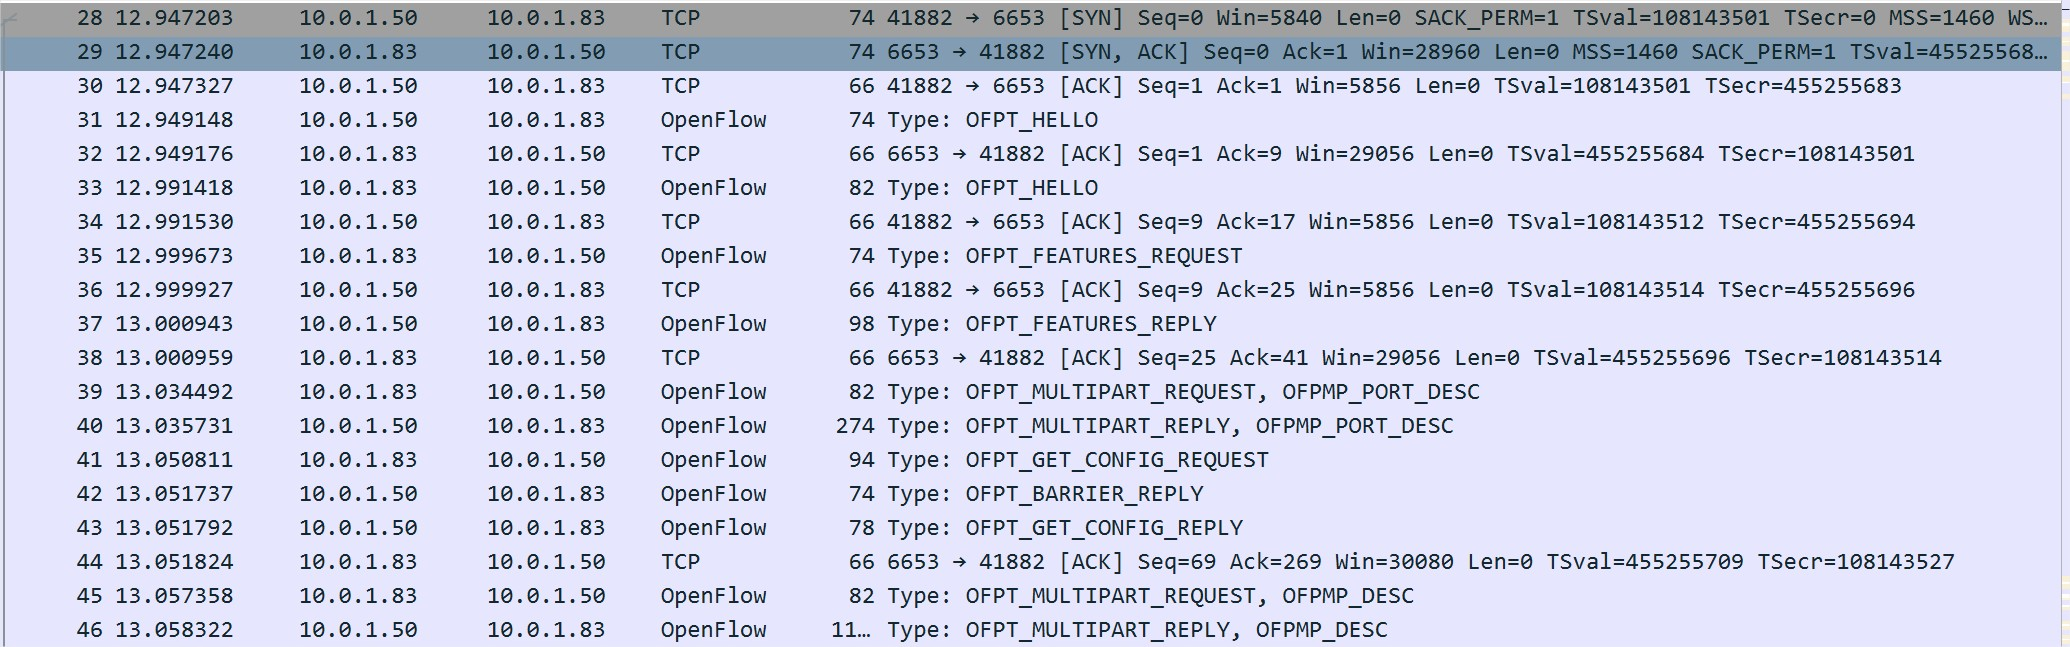
\includegraphics[scale=0.2]{images/floodlight.jpg}
    \caption{Wireshark - Start the controller}
    \label{fig:tolopogy}
\end{figure}


\begin{itemize}[noitemsep]
\item First a TCP session established between the switch and the controller
\item After that a Openflow Hello message send from the switch to the controller
\item The controller acknowledge the Hello message with a TCP ACK
\item The controller sends an Openflow Hello message back to the switch
\item The switch acknowledge the Hello message with a TCP ACK
\item After that the controller sends an OFPT\_FEATURES\_REQUEST message to the switch
\item The switch acknowledge the OFPT\_FEATURES\_REQUEST with a TCP ACK
\item The switch send the OFPT\_FEATURES\_REPLY message with the following parameters 
\end{itemize}

\begin{figure}[h]
    \centering
    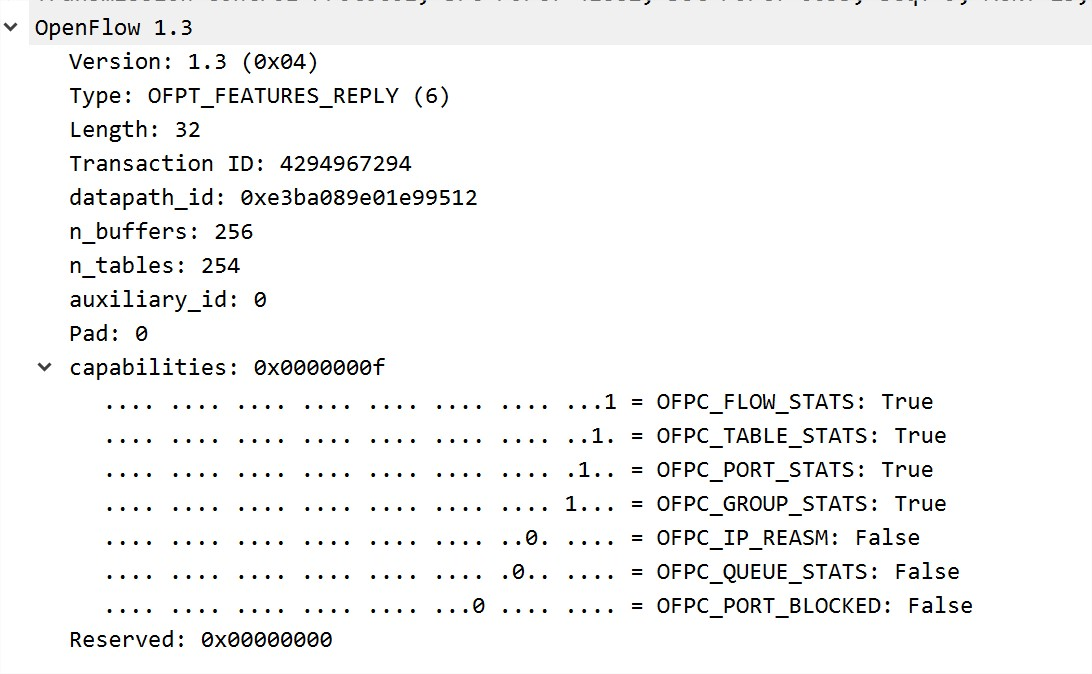
\includegraphics[scale=0.2]{images/OFPT_FEATURES_REPLY.jpg}
    \caption{Wireshark - OFPT\_FEATURES\_REPLY}
    \label{fig:tolopogy}
\end{figure}

\subsection{2- There are no flows in the switch and a new connection triggers a packet being sent to the controller.}

We started tshark again to capture the traffic on the interface between the switch and the controller. 
On Kotaiba's server (source IP 10.1.1.8) we started a ping to Fouad's server (destination IP 10.1.1.1)

\begin{figure}[h]
    \centering
    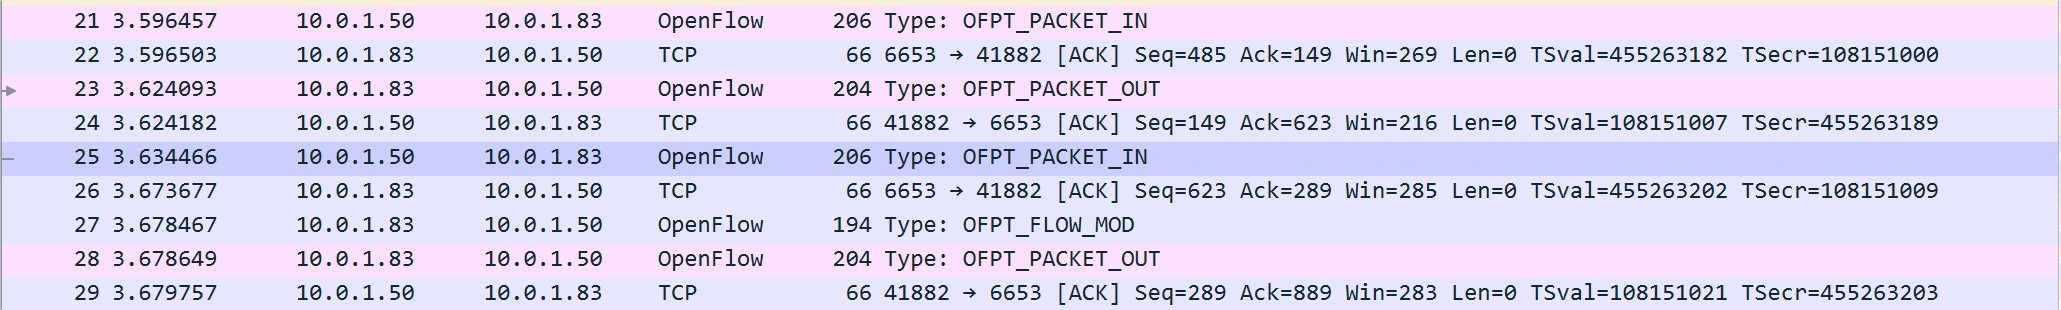
\includegraphics[scale=0.2]{images/ping.jpg}
    \caption{Wireshark - Pingt}
    \label{fig:tolopogy}
\end{figure}

The ping started at rule number 21.\\
The switch sends an OFPT\_PACKET\_IN packet to the controller with the ICMP REQUEST.

\begin{figure}[h]
    \centering
    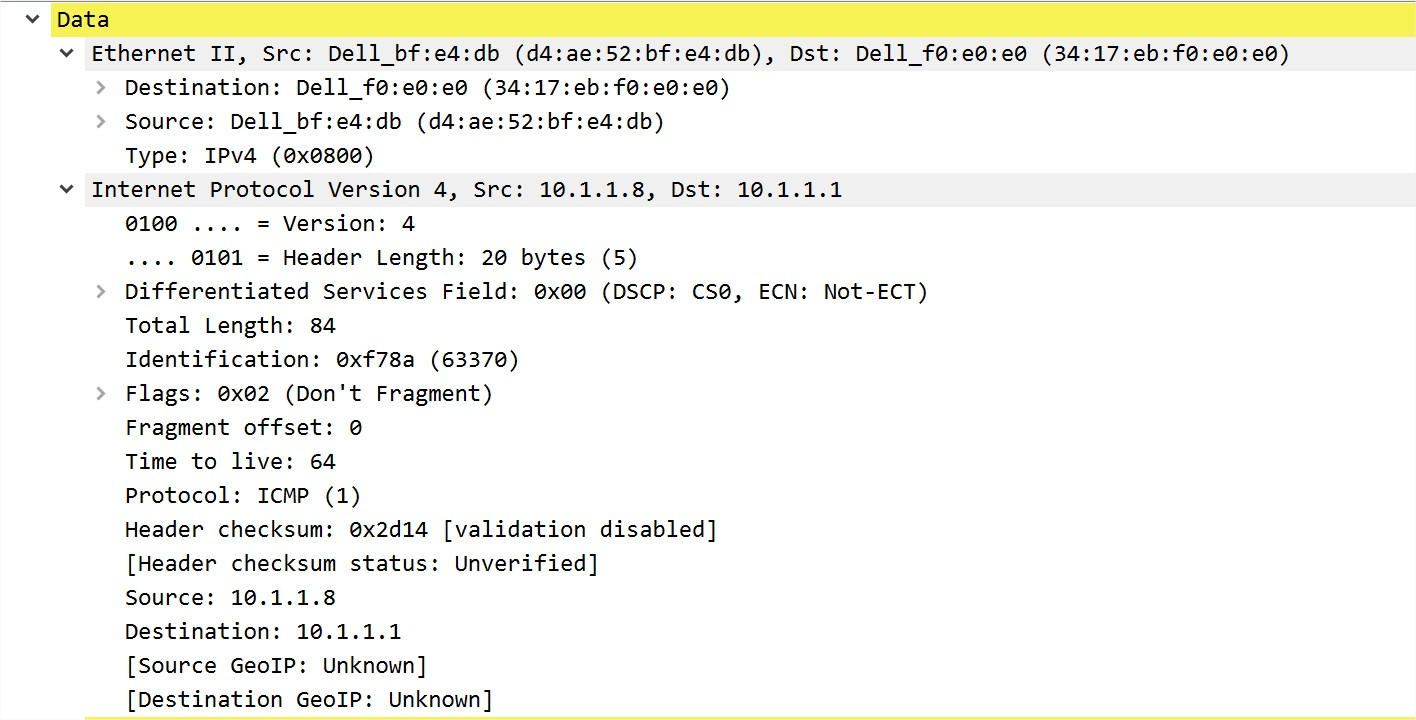
\includegraphics[scale=0.2]{images/ICMPREQUEST.jpg}
    \caption{Wireshark - ICMP REQUEST OFPT\_PACKET\_IN}
    \label{fig:ICMPREQUEST}
\end{figure}
\noindent
First the controller sends an ACK response followed with an OFPT\_PACKET\_OUT.  \\ In the OFPT\_PACKET\_OUT the controller sends the packet with an action to send the packet to Port: OFPD\_FLOOD. Which means to send the packet to "all physical ports, except the input port and those disabled by Spanning Tree Protocol."\cite{openflowactions} This is because the controller doesn't know yet after which port the IP address 10.1.1.1 is. \\
The switch acknowledged the packet with a TCP ACK message.\\
\begin{figure}[h]
    \centering
    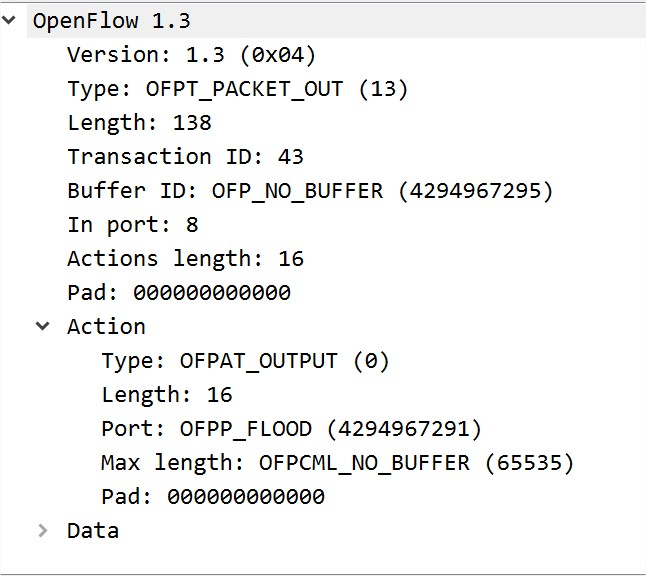
\includegraphics[scale=0.2]{images/ICMPREQUEST1.jpg}
    \caption{Wireshark - ICMP REQUEST OFPT\_PACKET\_OUT}
    \label{fig:ICMPREQUEST1}
\end{figure}
\noindent
Fouad's server sends a ICMP reply back to Kotaiba's server. This packet is first forwarded to the controller in an OFPT\_PACKET\_IN packet. The controller acknowledge the packet with a TCP ACK message. The controller defined a flow by sending an OFPT\_FLOW\_MOD message to the switch. After the flow is defined the controller send the packet to the switch with the action to send the packet to port 8 on the switch. 

\begin{figure}[h]
    \centering
    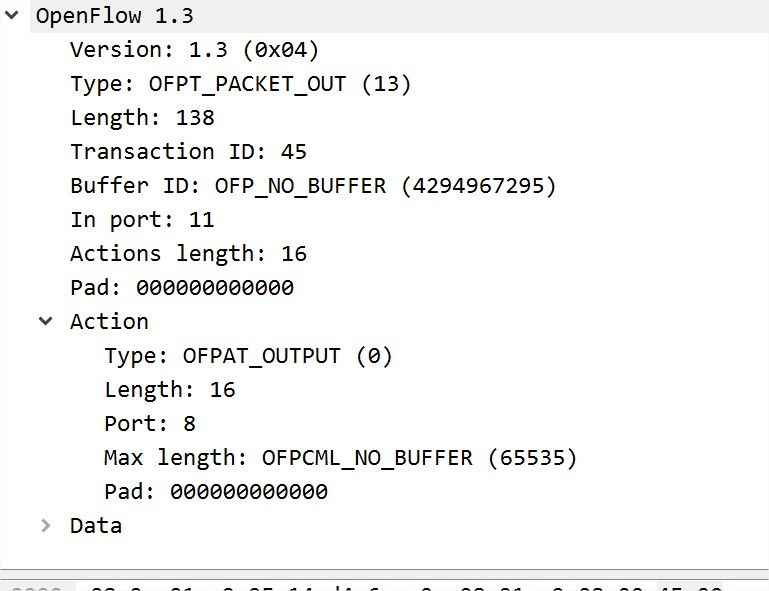
\includegraphics[scale=0.2]{images/ICMPREPLY.jpg}
    \caption{Wireshark - ICMP RELPY OFPT\_PACKET\_OUT}
    \label{fig:ICMPREPLY}
\end{figure}


\newpage
\section{Task 5: Static Flows}
\label{sec:task5}

Disable L2 switch:
\noindent
First,vwe remove the net.floodlightcontroller.forwarding.Forwarding line from src/main/resources/floodlightdefault.properties, after that we runned make command again. We checked with the following command if forwarding is still loaded.

\begin{verbatim}
curl http://127.0.0.1:8080/wm/core/module/all/json | jq
\end{verbatim}
\begin{verbatim}
  "net.floodlightcontroller.forwarding.Forwarding": {
    "loaded": false,
    "depends": {
      "net.floodlightcontroller.devicemanager.IDeviceService": "net.floodlightcontroller.devicemanager.internal.DeviceManagerImpl",
      "net.floodlightcontroller.topology.ITopologyService": "net.floodlightcontroller.topology.TopologyManager",
      "net.floodlightcontroller.routing.IRoutingService": "net.floodlightcontroller.topology.TopologyManager",
      "net.floodlightcontroller.core.IFloodlightProviderService": "net.floodlightcontroller.core.internal.Controller",
      "net.floodlightcontroller.debugcounter.IDebugCounterService": "net.floodlightcontroller.debugcounter.DebugCounterServiceImpl"
    },
    "provides": {}
  },
\end{verbatim}

Check if the ping is working:
\begin{verbatim}
root@bristol:~# ping 10.1.1.1
PING 10.1.1.1 (10.1.1.1) 56(84) bytes of data.
From 10.1.1.8 icmp_seq=9 Destination Host Unreachable
From 10.1.1.8 icmp_seq=10 Destination Host Unreachable
From 10.1.1.8 icmp_seq=11 Destination Host Unreachable
From 10.1.1.8 icmp_seq=12 Destination Host Unreachable
From 10.1.1.8 icmp_seq=13 Destination Host Unreachable
From 10.1.1.8 icmp_seq=14 Destination Host Unreachable
\end{verbatim}


Now, we are going to make the machines reachable again by pushing flows to the floodlight controller via its “staticflowpusher”
Web API:


From reims to bristol:

\begin{verbatim}
curl -X POST -d '{"switch":"e3:ba:08:9e:01:e9:95:12", "name":"flow1", 
"cookie":"0", "priority":"32768", "in_port":"11","active":"true","actions":"output=8"}' 
http://127.0.0.1:8080/wm/staticflowpusher/json
\end{verbatim}

From bristol to reims:

\begin{verbatim}
curl -X POST -d '{"switch":"e3:ba:08:9e:01:e9:95:12", "name":"flow2", 
"cookie":"0", "priority":"32768", "in_port":"8","active":"true","actions":"output=11"}' 
http://127.0.0.1:8080/wm/staticflowpusher/json
\end{verbatim}

Check, if its pushed:
\begin{verbatim}
curl http://127.0.0.1:8080/wm/staticflowpusher/list/e3:ba:08:9e:01:e9:95:12/json | jq
  % Total    % Received % Xferd  Average Speed   Time    Time     Time  Current
                                 Dload  Upload   Total   Spent    Left  Speed
100   613    0   613    0     0  14120      0 --:--:-- --:--:-- --:--:-- 14255
{
  "e3:ba:08:9e:01:e9:95:12": [
    {
      "flow1": {
        "version": "OF_13",
        "command": "ADD",
        "cookie": "45035998409453772",
        "priority": "-32768",
        "idleTimeoutSec": "0",
        "hardTimeoutSec": "0",
        "outPort": "any",
        "flags": "1",
        "cookieMask": "0",
        "outGroup": "any",
        "match": {
          "in_port": "11"
        },
        "instructions": {
          "instruction_apply_actions": {
            "actions": "output=8"
          }
        }
      }
    },
    {
      "flow2": {
        "version": "OF_13",
        "command": "ADD",
        "cookie": "45035998409453773",
        "priority": "-32768",
        "idleTimeoutSec": "0",
        "hardTimeoutSec": "0",
        "outPort": "any",
        "flags": "1",
        "cookieMask": "0",
        "outGroup": "any",
        "match": {
          "in_port": "8"
        },
        "instructions": {
          "instruction_apply_actions": {
            "actions": "output=11"
          }
        }
      }
    }
  ]
}
\end{verbatim}


Check ping now, its working:
\begin{verbatim}
root@bristol:~# ping 10.1.1.1
PING 10.1.1.1 (10.1.1.1) 56(84) bytes of data.
64 bytes from 10.1.1.1: icmp_seq=1 ttl=64 time=0.194 ms
64 bytes from 10.1.1.1: icmp_seq=2 ttl=64 time=0.170 ms
64 bytes from 10.1.1.1: icmp_seq=3 ttl=64 time=0.174 ms
\end{verbatim}

\subsection{Show that the machines can reach each other?}


\section{Task 6: VLAN translation}
\label{sec:task3}
We first installed vlan and created a vlan on eno2 assign an ip address to the vlan an set the interface up.
Fouad's server
\begin{verbatim}
sudo apt-get install vlan
sudo modprobe 8021q
sudo vconfig add eno2 11
Added VLAN with VID == 11 to IF -:eno2:-
sudo ip addr add 10.11.1.1/24 dev eno2.11
sudo ip link set up eno2.11
\end{verbatim}

Kotaiba's server
\begin{verbatim}
sudo apt-get install vlan
sudo modprobe 8021q
sudo vconfig add eno2 8
Added VLAN with VID == 8 to IF -:eno2:-
sudo ip addr add 10.11.1.2/24 dev eno2.8
sudo ip link set up eno2.8 
\end{verbatim}
\noindent
To let OpenFlow switch doing the VLAN translation we needed to configure two flows in the OpenFlow switch. The first flow to translate all incoming traffic from port ge-1/1/11 with tagged traffic of vlan 11 to port ge-1/1/8 into vlan 8 and another rule the other way around.

\begin{verbatim}
curl -X POST -d '{"switch":"e3:ba:08:9e:01:e9:95:12", "name":"flow3", "cookie":"0", "priority":"32768", 
"in_port":"11","eth_vlan_pcp":"0","eth_vlan_vid":"0x0B","active":"true","actions":"set_field=eth_vlan_pcp->0,
set_field=eth_vlan_vid->8,output=8"}' http://127.0.0.1:8080/wm/staticflowpusher/json

curl -X POST -d '{"switch":"e3:ba:08:9e:01:e9:95:12", "name":"flow4", "cookie":"0", "priority":"32768", 
"in_port":"8","eth_vlan_pcp":"0","eth_vlan_vid":"0x08","active":"true","actions":"set_field=eth_vlan_pcp->0,
set_field=eth_vlan_vid->11,output=11"}' http://127.0.0.1:8080/wm/staticflowpusher/json
\end{verbatim}


output of the current flows in Floodlight
\begin{verbatim}
fmakioui@reims:~$ curl http://127.0.0.1:8080/wm/staticflowpusher/list/all/json | jq
  % Total    % Received % Xferd  Average Speed   Time    Time     Time  Current
                                 Dload  Upload   Total   Spent    Left  Speed
100   730    0   730    0     0   213k      0 --:--:-- --:--:-- --:--:--  237k
{
  "e3:ba:08:9e:01:e9:95:12": [
    {
      "flow3": {
        "version": "OF_13",
        "command": "ADD",
        "cookie": "45035998409453774",
        "priority": "-32768",
        "idleTimeoutSec": "0",
        "hardTimeoutSec": "0",
        "outPort": "any",
        "flags": "1",
        "cookieMask": "0",
        "outGroup": "any",
        "match": {
          "in_port": "11",
          "eth_vlan_vid": "0xb",
          "eth_vlan_pcp": "0x0"
        },
        "instructions": {
          "instruction_apply_actions": {
            "actions": ",eth_vlan_vid=8,output=8"
          }
        }
      }
    },
    {
      "flow4": {
        "version": "OF_13",
        "command": "ADD",
        "cookie": "45035998409453775",
        "priority": "-32768",
        "idleTimeoutSec": "0",
        "hardTimeoutSec": "0",
        "outPort": "any",
        "flags": "1",
        "cookieMask": "0",
        "outGroup": "any",
        "match": {
          "in_port": "8",
          "eth_vlan_vid": "0x8",
          "eth_vlan_pcp": "0x0"
        },
        "instructions": {
          "instruction_apply_actions": {
            "actions": ",eth_vlan_vid=11,output=11"
          }
        }
      }
    }
  ]
}

\end{verbatim}

Test that the rules are working

\begin{verbatim}
ping 10.11.1.2
PING 10.11.1.2 (10.11.1.2) 56(84) bytes of data.
64 bytes from 10.11.1.2: icmp_seq=1 ttl=64 time=0.204 ms
64 bytes from 10.11.1.2: icmp_seq=2 ttl=64 time=0.180 ms
64 bytes from 10.11.1.2: icmp_seq=3 ttl=64 time=0.217 ms

\end{verbatim}


\newpage
\section{Task 7: Traffic firewalling}

We are going to team up with (Peter Prj and Henri).

Servers used:
\begin{verbatim}
    Server-1: 10.1.1.1 % Fouad server on interface 11 MAC 34:17:eb:f0:e0:e0
    Server-2: 10.1.1.2 % Henri server on interface 1 MAC  34:17:eb:f0:e0:64 
    Server-3: 10.1.1.3 % Peter server on interface 2 MAC 34:17:eb:ec:20:47 
    Server-4: 10.1.1.8 % Kotaiba server on interface 8 MAC d4:ae:52:bf:e4:db
\end{verbatim}

Create the following scenario using the static flow pusher:

First, put all of the switch ports in the same virtual switch.
\begin{verbatim}
ovs-vsctl add-br br_11_5 -- set bridge br_11_5 datapath_type=pica8
ovs-vsctl del-br br_11
ovs-vsctl del-br br_5
ovs-vsctl add-port br_11_5 ge-1/1/11 vlan_mode=trunk -- set interface ge-1/1/11 type=pica8
ovs-vsctl add-port br_11_5 ge-1/1/8 vlan_mode=trunk -- set interface ge-1/1/8 type=pica8
ovs-vsctl add-port br_11_5 ge-1/1/2 vlan_mode=trunk -- set interface ge-1/1/2 type=pica8
ovs-vsctl add-port br_11_5 ge-1/1/1 vlan_mode=trunk -- set interface ge-1/1/1 type=pica8
ovs-vsctl set-controller br_5 tcp:10.0.1.222:6653 % Peter's management interface
\end{verbatim}

\begin{verbatim}
Switch MAC address: 0e:39:08:9e:01:e9:95:12

curl -X POST -d '{"switch":"0e:39:08:9e:01:e9:95:12", "name":"AllowARP", "cookie":"0", "priority":"32768", "eth_type":"0x806","active":"true","actions":"output=11,output=2,output=1,output=8"}' http://127.0.0.1:8080/wm/staticflowpusher/json


curl -X POST -d '{"switch":"0e:39:08:9e:01:e9:95:12", "name":"Peter_to_Fouad_MAC", "cookie":"0", "priority":"32768", "in_port": "2","eth_src":"34:17:eb:ec:20:47", "eth_dst":"34:17:eb:f0:e0:e0","active":"true","actions":"output=11"}' http://127.0.0.1:8080/wm/staticflowpusher/json


curl -X POST -d '{"switch":"0e:39:08:9e:01:e9:95:12", "name":"Kotaiba_to_Fouad_MAC", "cookie":"0", "priority":"32768", "in_port": "8","eth_src":"d4:ae:52:bf:e4:db", "eth_dst":"34:17:eb:f0:e0:e0", "active":"true","actions":"output=11"}' http://127.0.0.1:8080/wm/staticflowpusher/json


curl -X POST -d '{"switch":"0e:39:08:9e:01:e9:95:12", "name":"Peter_to_Henri_IP","cookie":"0", "priority":"32768","in_port": "2","eth_type":"2048", "ipv4_src":"10.1.1.3", "ipv4_dst":"10.1.1.2","active":"true","actions":"output=1"}' http://127.0.0.1:8080/wm/staticflowpusher/json


curl -X POST -d '{"switch":"0e:39:08:9e:01:e9:95:12", "name":"Kotaiba_to_Henri_TCP_MAC", "cookie":"0", "priority":"32768","in_port": "8", "eth_type":"2048", "eth_src":"d4:ae:52:bf:e4:db", "eth_dst":"34:17:eb:f0:e0:64", "ip_proto":"0x06","tcp_dst":"80", "active":"true","actions":"output=1"}' http://127.0.0.1:8080/wm/staticflowpusher/json

curl -X POST -d '{"switch":"0e:39:08:9e:01:e9:95:12", "name":"Henri_to_Peter_HTTP", "cookie":"0", "priority":"32768", "eth_type":"2048", "in_port":"1", "ipv4_dst":"10.1.1.3", "ip_proto":"0x06","tcp_dst":"80", "active":"true","actions":"output=2"}' http://127.0.0.1:8080/wm/staticflowpusher/json

curl -X POST -d '{"switch":"0e:39:08:9e:01:e9:95:12", "name":"Kotaiba_to_Peter_MAC", "cookie":"0", "priority":"32768","in_port": "8", "eth_src":"d4:ae:52:bf:e4:db", "eth_dst":"34:17:eb:ec:20:47", "active":"true","actions":"output=2"}' http://127.0.0.1:8080/wm/staticflowpusher/json


curl -X POST -d '{"switch":"0e:39:08:9e:01:e9:95:12", "name":"Fouad_to_Peter_IP", "cookie":"0", "priority":"32768","in_port": "11", "eth_type":"2048", "ipv4_src":"10.1.1.1", "ipv4_dst":"10.1.1.3", "active":"true","actions":"output=2"}' http://127.0.0.1:8080/wm/staticflowpusher/json


curl -X POST -d '{"switch":"0e:39:08:9e:01:e9:95:12", "name":"Peter_to_Kotaiba_MAC", "cookie":"0", "priority":"32768","in_port": "2", "eth_src":"34:17:eb:ec:20:47", "eth_dst":"d4:ae:52:bf:e4:db", "active":"true","actions":"output=8"}' http://127.0.0.1:8080/wm/staticflowpusher/json


curl -X POST -d '{"switch":"0e:39:08:9e:01:e9:95:12", "name":"Fouad_to_Peter_SSH", "cookie":"0", "priority":"32768","in_port": "11", "eth_src":"34:17:eb:f0:e0:e0", "eth_type":"2048", "ipv4_dst":"10.1.1.8", "eth_type":"2048", "ip_proto":"0x06","tcp_dst":"22", "active":"true","actions":"output=8"}' http://127.0.0.1:8080/wm/staticflowpusher/json


curl -X POST -d '{"switch":"0e:39:08:9e:01:e9:95:12", "name":"Henri_to_Kotaiba_IP", "cookie":"0", "priority":"32768","in_port": "1", "eth_type":"2048", "ipv4_src":"10.1.1.2", "ipv4_dst":"10.1.1.8", "active":"true","actions":"output=8"}' http://127.0.0.1:8080/wm/staticflowpusher/json


curl http://127.0.0.1:8080/wm/staticflowpusher/list/0e:39:08:9e:01:e9:95:12/json | jq


 
root@bordeaux:/etc# curl http://127.0.0.1:8080/wm/staticflowpusher/list/0e:39:08:9e:01:e9:95:12/json | jq
  % Total    % Received % Xferd  Average Speed   Time    Time     Time  Current
                                 Dload  Upload   Total   Spent    Left  Speed
100  4142    0  4142    0     0   226k      0 --:--:-- --:--:-- --:--:--  237k
{
  "0e:39:08:9e:01:e9:95:12": [
    {
      "Peter_to_Kotaiba_MAC": {
        "version": "OF_13",
        "command": "ADD",
        "cookie": "45035996874724473",
        "priority": "-32768",
        "idleTimeoutSec": "0",
        "hardTimeoutSec": "0",
        "outPort": "any",
        "flags": "1",
        "cookieMask": "0",
        "outGroup": "any",
        "match": {
          "in_port": "2",
          "eth_dst": "d4:ae:52:bf:e4:db",
          "eth_src": "34:17:eb:ec:20:47"
        },
        "instructions": {
          "instruction_apply_actions": {
            "actions": "output=8"
          }
        }
      }
    },
    {
      "Peter_to_Henri_IP": {
        "version": "OF_13",
        "command": "ADD",
        "cookie": "45035996466963196",
        "priority": "-32768",
        "idleTimeoutSec": "0",
        "hardTimeoutSec": "0",
        "outPort": "any",
        "flags": "1",
        "cookieMask": "0",
        "outGroup": "any",
        "match": {
          "in_port": "2",
          "eth_type": "0x0x800",
          "ipv4_src": "10.1.1.3",
          "ipv4_dst": "10.1.1.2"
        },
        "instructions": {
          "instruction_apply_actions": {
            "actions": "output=1"
          }
        }
      }
    },
    {
      "Peter_to_Fouad_MAC": {
        "version": "OF_13",
        "command": "ADD",
        "cookie": "45035997466145553",
        "priority": "-32768",
        "idleTimeoutSec": "0",
        "hardTimeoutSec": "0",
        "outPort": "any",
        "flags": "1",
        "cookieMask": "0",
        "outGroup": "any",
        "match": {
          "in_port": "2",
          "eth_dst": "34:17:eb:f0:e0:e0",
          "eth_src": "34:17:eb:ec:20:47"
        },
        "instructions": {
          "instruction_apply_actions": {
            "actions": "output=11"
          }
        }
      }
    },
    {
      "Fouad_to_Peter_IP": {
        "version": "OF_13",
        "command": "ADD",
        "cookie": "45035997708743759",
        "priority": "-32768",
        "idleTimeoutSec": "0",
        "hardTimeoutSec": "0",
        "outPort": "any",
        "flags": "1",
        "cookieMask": "0",
        "outGroup": "any",
        "match": {
          "in_port": "11",
          "eth_type": "0x0x800",
          "ipv4_src": "10.1.1.1",
          "ipv4_dst": "10.1.1.3"
        },
        "instructions": {
          "instruction_apply_actions": {
            "actions": "output=2"
          }
        }
      }
    },
    {
      "AllowARP": {
        "version": "OF_13",
        "command": "ADD",
        "cookie": "45035997712420157",
        "priority": "-32768",
        "idleTimeoutSec": "0",
        "hardTimeoutSec": "0",
        "outPort": "any",
        "flags": "1",
        "cookieMask": "0",
        "outGroup": "any",
        "match": {
          "eth_type": "0x0x806"
        },
        "instructions": {
          "instruction_apply_actions": {
            "actions": "output=11,output=2,output=1,output=8"
          }
        }
      }
    },
    {
      "Henri_to_Peter_HTTP": {
        "version": "OF_13",
        "command": "ADD",
        "cookie": "45035999333422241",
        "priority": "-32768",
        "idleTimeoutSec": "0",
        "hardTimeoutSec": "0",
        "outPort": "any",
        "flags": "1",
        "cookieMask": "0",
        "outGroup": "any",
        "match": {
          "in_port": "1",
          "eth_type": "0x0x800",
          "ip_proto": "0x6",
          "ipv4_dst": "10.1.1.3",
          "tcp_dst": "80"
        },
        "instructions": {
          "instruction_apply_actions": {
            "actions": "output=2"
          }
        }
      }
    },
    {
      "Kotaiba_to_Henri_TCP_MAC": {
        "version": "OF_13",
        "command": "ADD",
        "cookie": "45035997310784857",
        "priority": "-32768",
        "idleTimeoutSec": "0",
        "hardTimeoutSec": "0",
        "outPort": "any",
        "flags": "1",
        "cookieMask": "0",
        "outGroup": "any",
        "match": {
          "in_port": "8",
          "eth_dst": "34:17:eb:f0:e0:64",
          "eth_src": "d4:ae:52:bf:e4:db",
          "eth_type": "0x0x800",
          "ip_proto": "0x6",
          "tcp_dst": "80"
        },
        "instructions": {
          "instruction_apply_actions": {
            "actions": "output=1"
          }
        }
      }
    },
    {
      "Henri_to_Kotaiba_IP": {
        "version": "OF_13",
        "command": "ADD",
        "cookie": "45035998353712421",
        "priority": "-32768",
        "idleTimeoutSec": "0",
        "hardTimeoutSec": "0",
        "outPort": "any",
        "flags": "1",
        "cookieMask": "0",
        "outGroup": "any",
        "match": {
          "in_port": "1",
          "eth_type": "0x0x800",
          "ipv4_src": "10.1.1.2",
          "ipv4_dst": "10.1.1.8"
        },
        "instructions": {
          "instruction_apply_actions": {
            "actions": "output=8"
          }
        }
      }
    },
    {
      "Fouad_to_Peter_SSH": {
        "version": "OF_13",
        "command": "ADD",
        "cookie": "45035998419626744",
        "priority": "-32768",
        "idleTimeoutSec": "0",
        "hardTimeoutSec": "0",
        "outPort": "any",
        "flags": "1",
        "cookieMask": "0",
        "outGroup": "any",
        "match": {
          "in_port": "11",
          "eth_src": "34:17:eb:f0:e0:e0",
          "eth_type": "0x0x800",
          "ip_proto": "0x6",
          "ipv4_dst": "10.1.1.8",
          "tcp_dst": "22"
        },
        "instructions": {
          "instruction_apply_actions": {
            "actions": "output=8"
          }
        }
      }
    },
    {
      "Kotaiba_to_Fouad_MAC": {
        "version": "OF_13",
        "command": "ADD",
        "cookie": "45035999513130890",
        "priority": "-32768",
        "idleTimeoutSec": "0",
        "hardTimeoutSec": "0",
        "outPort": "any",
        "flags": "1",
        "cookieMask": "0",
        "outGroup": "any",
        "match": {
          "in_port": "8",
          "eth_dst": "34:17:eb:f0:e0:e0",
          "eth_src": "d4:ae:52:bf:e4:db"
        },
        "instructions": {
          "instruction_apply_actions": {
            "actions": "output=11"
          }
        }
      }
    },
    {
      "Kotaiba_to_Peter_MAC": {
        "version": "OF_13",
        "command": "ADD",
        "cookie": "45035999807353863",
        "priority": "-32768",
        "idleTimeoutSec": "0",
        "hardTimeoutSec": "0",
        "outPort": "any",
        "flags": "1",
        "cookieMask": "0",
        "outGroup": "any",
        "match": {
          "in_port": "8",
          "eth_dst": "34:17:eb:ec:20:47",
          "eth_src": "d4:ae:52:bf:e4:db"
        },
        "instructions": {
          "instruction_apply_actions": {
            "actions": "output=2"
          }
        }
      }
    }
  ]
}



\end{verbatim}


• Fouad can SSH to Kotaiba's server
\begin{verbatim}
fmakioui@reims:~$ ssh fouad@10.1.1.8
The authenticity of host '10.1.1.8 (10.1.1.8)' can't be established.
ECDSA key fingerprint is SHA256:Vrs17X1WQXR9kK3KxVqhCdO719kiMtXLIMbDCbCyQ14.
Are you sure you want to continue connecting (yes/no)? yes
Warning: Permanently added '10.1.1.8' (ECDSA) to the list of known hosts.
fouad@10.1.1.8's password:
Welcome to Ubuntu 16.04.4 LTS (GNU/Linux 4.4.0-112-generic x86_64)

 * Documentation:  https://help.ubuntu.com
 * Management:     https://landscape.canonical.com
 * Support:        https://ubuntu.com/advantage
Last login: Wed Mar 14 17:10:12 2018 from 145.100.104.122
fouad@bristol:~$
\end{verbatim}


• Fouad can ping Peter's server 
\begin{verbatim}
fmakioui@reims:~$ ping 10.1.1.3
PING 10.1.1.3 (10.1.1.3) 56(84) bytes of data.
64 bytes from 10.1.1.3: icmp_seq=1 ttl=64 time=0.385 ms
64 bytes from 10.1.1.3: icmp_seq=2 ttl=64 time=0.172 ms
^C
--- 10.1.1.3 ping statistics ---
2 packets transmitted, 2 received, 0% packet loss, time 1000ms
rtt min/avg/max/mdev = 0.172/0.278/0.385/0.107 ms
fmakioui@reims:~$ 
\end{verbatim}


• Henri can perform HTTP requests to Peter's server
\begin{verbatim}
root@calais:/var/www/html # curl 10.1.1.3

<!DOCTYPE html PUBLIC "-//W3C//DTD XHTML 1.0 Transitional//EN" "http://www.w3.org/TR/xhtml1/DTD/xhtml1-transitional.dtd">
<html xmlns="http://www.w3.org/1999/xhtml">
  <!--
\
\end{verbatim}


• Peter can SSH to Kotaiba's server
\begin{verbatim}
root@bordeaux:/etc# ssh 10.1.1.8
root@10.1.1.8's password: 
Permission denied, please try again.
root@10.1.1.8's password: 
Permission denied, please try again.
root@10.1.1.8's password: 
Permission denied (publickey,password).
\end{verbatim}



• Server 4 can perform HTTP requests to server 2
\begin{verbatim}
    root@bristol:~# curl 10.1.1.2
<!DOCTYPE html>
<html>
	<?php echo "Ceci est du texte"; ?>
    <head>
        <title>Notre première instruction : echo</title>
        <meta charset="utf-8" />
    </head>
    <body>
        <h2>Affichage de texte avec PHP</h2>
	<img src="output.png">        
        <p>
            Cette ligne a été écrite entièrement en HTML.<br />
	</p>
            <?php echo "Celle-ci a ete�ecrite entierement en PHP."; ?>
    </body>
</html>
\end{verbatim}


\textbf{Check the flow table:}

\begin{verbatim}
 ovs-ofctl dump-flows br_11_5
 OFPST_FLOW reply (OF1.4) (xid=0x2):
 cookie=0xa000003dd09559, duration=262.367s, table=0, n_packets=n/a, n_bytes=500, send_flow_rem tcp,in_port=8,dl_src=d4:ae:52:bf:e4:db,dl_dst=34:17:eb:f0:e0:64,tp_dst=80 actions=output:1
 cookie=0xa000005588f44f, duration=262.323s, table=0, n_packets=n/a, n_bytes=204, send_flow_rem ip,in_port=11,nw_src=10.1.1.1,nw_dst=10.1.1.3 actions=output:2
 cookie=0xa000000b84e2fc, duration=262.412s, table=0, n_packets=n/a, n_bytes=12354, send_flow_rem ip,in_port=2,nw_src=10.1.1.3,nw_dst=10.1.1.2 actions=output:1
 cookie=0xa000007bfa6525, duration=262.263s, table=0, n_packets=n/a, n_bytes=978, send_flow_rem ip,in_port=1,nw_src=10.1.1.2,nw_dst=10.1.1.8 actions=output:8
 cookie=0xa0000055c10d3d, duration=262.482s, table=0, n_packets=n/a, n_bytes=52608, send_flow_rem arp actions=output:11,output:2,output:1,output:8
 cookie=0xa00000c115b78a, duration=262.433s, table=0, n_packets=n/a, n_bytes=5471, send_flow_rem in_port=8,dl_src=d4:ae:52:bf:e4:db,dl_dst=34:17:eb:f0:e0:e0 actions=output:11
 cookie=0xa0000023d2d479, duration=262.300s, table=0, n_packets=n/a, n_bytes=3577, send_flow_rem in_port=2,dl_src=34:17:eb:ec:20:47,dl_dst=d4:ae:52:bf:e4:db actions=output:8
 cookie=0xa0000047133311, duration=262.453s, table=0, n_packets=n/a, n_bytes=204, send_flow_rem in_port=2,dl_src=34:17:eb:ec:20:47,dl_dst=34:17:eb:f0:e0:e0 actions=output:11
 cookie=0xa00000d29f3407, duration=262.342s, table=0, n_packets=n/a, n_bytes=2813, send_flow_rem in_port=8,dl_src=d4:ae:52:bf:e4:db,dl_dst=34:17:eb:ec:20:47 actions=output:2
 cookie=0x0, duration=283.738s, table=0, n_packets=n/a, n_bytes=64, priority=0 actions=CONTROLLER:65535
 cookie=0xa00000b65f94a1, duration=262.363s, table=0, n_packets=n/a, n_bytes=570, send_flow_rem tcp,in_port=1,nw_dst=10.1.1.3,tp_dst=80 actions=output:2
 cookie=0xa000007fe82af8, duration=262.278s, table=0, n_packets=n/a, n_bytes=5529, send_flow_rem tcp,in_port=11,dl_src=34:17:eb:f0:e0:e0,nw_dst=10.1.1.8,tp_dst=22 actions=output:8   
\end{verbatim}]
 

\label{sec:task3}

\newpage
\bibliographystyle{plain}
\bibliography{references}
\end{document}